\begin{surferPage}{Flater med mange reelle singulariteter}
    Som nevnt tidligere, vet vi ikke det nøyaktige antallet 
    $\mu(7)$ av singulariteter på en flate av sjuende grad.
    Vi har bare en øvre og en nedre grense: $99\le \mu(7) \le 104$. 

	Derfor er det ikke så overraskende at man vet enda mindre om flater med en generell grad $d$.
	
	Sonja Breske, Oliver Labs og Duco van Straten har i det minste lyktes med å endre på en konstruksjon 
	av S. V. \ Chmutov, slik at det nåværende maksimale antallet
	singulariteter også er oppnådd for flater med reelle singulariteter. Til nå vet vi:
 
    \[0,41\bar{6}d^3 \lessapprox \mu(d) \lessapprox 0.44\bar{4} d^3.\]
Fra intervallet over kan man se symmetrien til konstruksjonen og en relasjon til det maksimale antallet sorte celler i et arrangement av linjer:
    \begin{center}
      \begin{tabular}{c@{\qquad}c}
        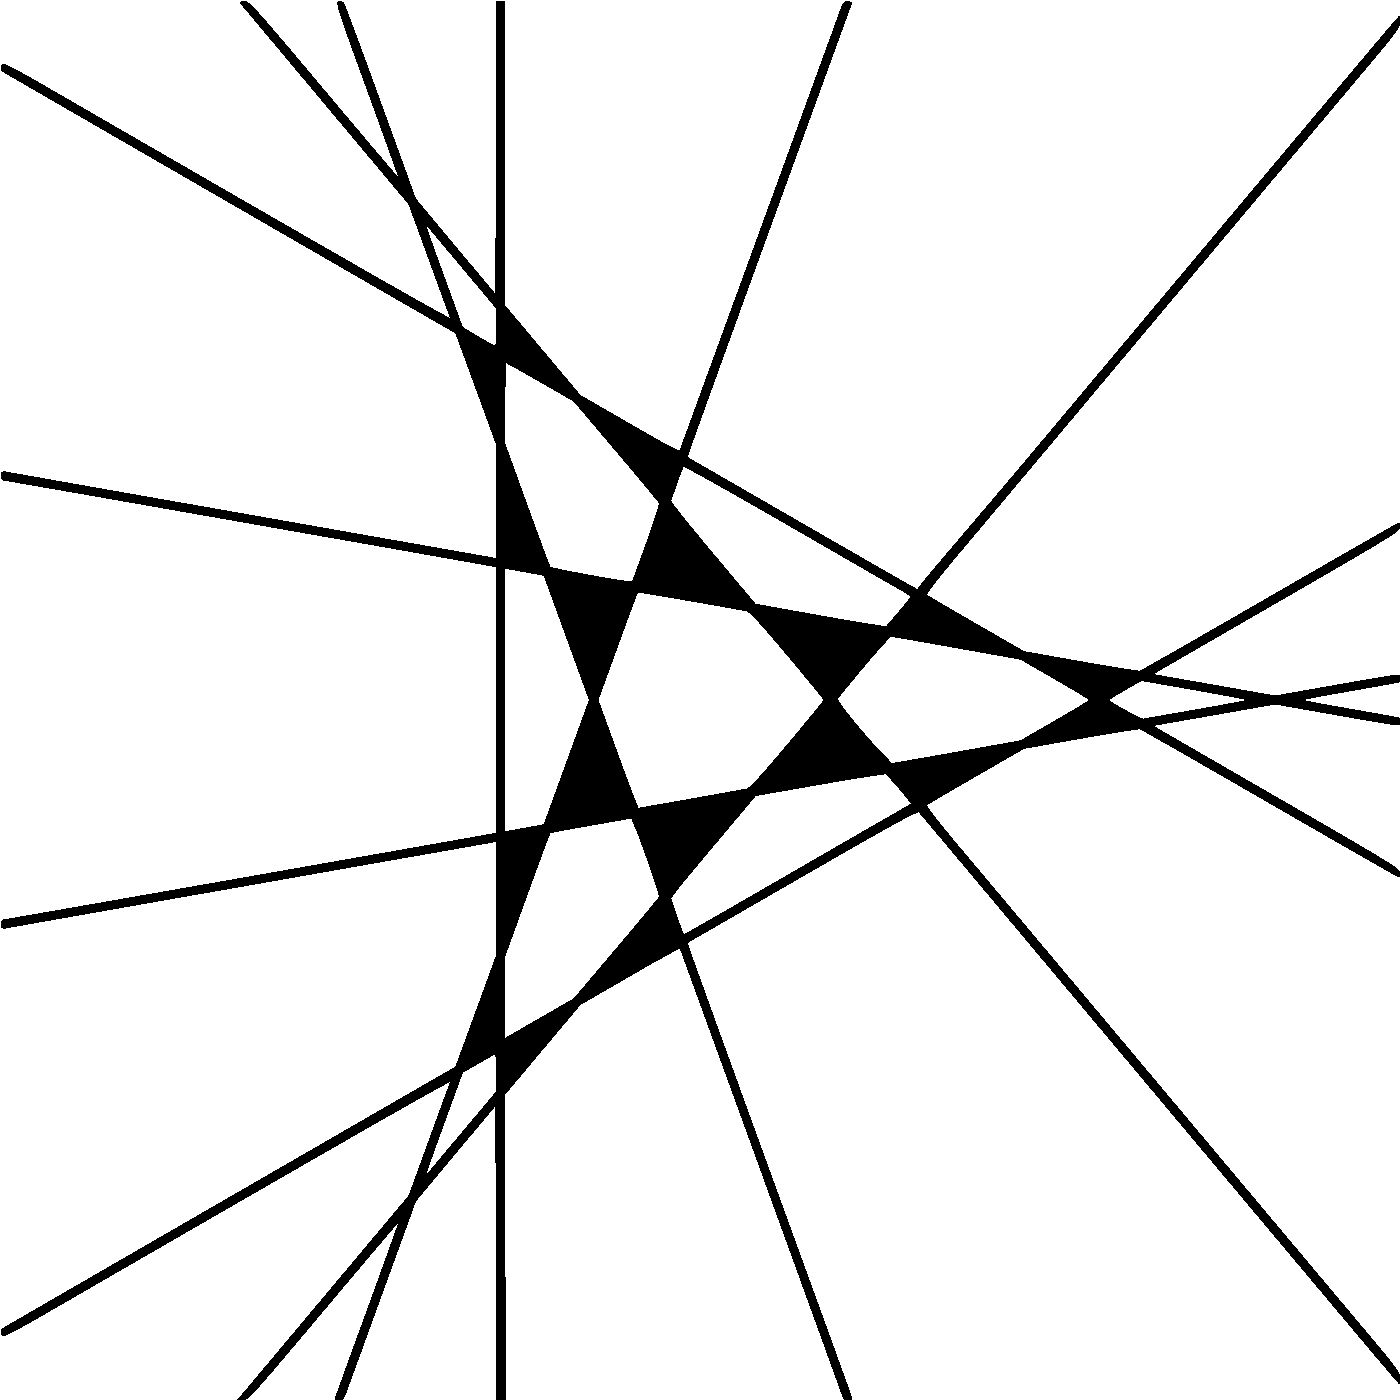
\includegraphics[height=1.5cm]{./../../common/images/vielesing.pdf}
        &
        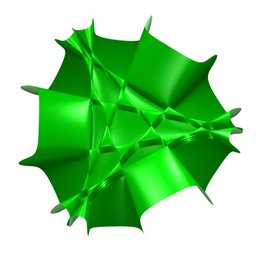
\includegraphics[height=1.5cm]{./../../common/images/p9surface_von_oben}
      \end{tabular}
    \end{center}
\end{surferPage}
